\section{Supporting Flyspeck in a Semantic Wiki (Christoph)}

Starting from requirements how collaborating on formalizing the Kepler proof should be
supported, we have evaluated the applicability of two concrete semantic wikis to Flyspeck
in order to see what possibilities this technology can offer for the project:  our own
semantic wiki SWiM, and a rapid prototype developed on top of Semantic MediaWiki.  Based on the
results of this pre-study, we establish a roadmap for tailoring SWiM to specifically meet
the needs of the Flyspeck collaborators.

\subsection{Workflow Requirements (Christoph, Sean)}
\label{sec:req}

So far, the Flyspeck project has had two\ednote{@Sean, fix the number!} core members who
collaborated via Google Code~\cite{flyspeck:web}.  While the services offered by Google
Code (a Subversion repository, a mailing list, and others) were found to be sufficient for
the core development team, we were not satisfied with the wiki integrated into the Google
Code web interface.  Lacking support for mathematical formulae, it would not even allow
for presenting the theorems and lemmas to be formally proved in a human-readable fashion.
Secondly, besides untyped links and adding labels to pages it does not offer any further
\emph{structuring} support, which we found essential for browsing and querying Flyspeck's
large knowledge collection.

In this early phase of ``crowdsourcing'' Flyspeck, the focus is not yet on developing and
checking formal proofs collaboratively, but on making its extent and structure
comprehensible and on communicating where work needs to be done.  For this the outline of
the whole proof from the book\ednote{@Sean, I guess I should assume that you introduce the
  book in the Flyspeck intro. --CL} needs to be represented in the wiki, where the
mathematical statements (including definitions, lemmas, and theorems) are available in a
human-readable way (with formulae in \LaTeX\ or presentational MathML) as well as a
machine-readable presentation suitable for downloading into a theorem prover.  In order to
obtain a well-structured network of knowledge items, each mathematical statement should be
presented on one wiki page, which shows its human-readable representation from the book,
offers additional space for annotation, and allows for downloading a formal
representation.  We considered the following kinds of annotations desirable:

\begin{description}
\item[Categorization by topic:] In the beginning, one would mirror the narrative structure
  of the book (e.\,g.\ ``ball'' being a subsection of ``primitive volumes'', which in turn
  is a section of the chapter ``volume calculations'').  Standardized ways of classifying
  mathematical topics, such as the Mathematical Subject Classification
  (MSC)~\cite{AMS:MSC2000}, could be added later.
\item[Project-organization metadata] such as the information whether a lemma has already
  been proven formally, or in what theorem proving language there are proof objects
  available.\ednote{@Sean: more?}
\item[Dependency links:] These can be links from individual symbols in mathematical
  formulae to the place where they are declared, or from any page $p$ to other pages
  containing knowledge that is required for understanding $p$ --- either pages in the same
  wiki, or external resources like PlanetMath or Wikipedia articles.
\item[Discussion posts] should be strongly tied to the topic being discussed, and they
  should be classified into categories like question, answer, explanation,
  etc.
\end{description}

To the visitor and potential collaborator, an impression of the extent and structure of
the project --- its enourmous size and its specialization into diverse fields of
mathematics --- must be given, as well as tools for browsing and querying the knowledge.
The topical structure as well as the dependencies must be browsable via links.  Not only
should it be possible to query knowledge items by their annotations, but important query
results must also be available as dynamically generated lists.  Examples for queries are:

\begin{enumerate}
\item\label{item:proven-lemma} ``Which lemmas about composite regions have not been
  formally proven so far?''
\item ``What do I need to read in order to understand Jordan's curve
  theorem?''\ednote{internal dependency graph, tutorial, planetmath}
\item ``What lemmas are difficult to prove?''
  \begin{enumerate}
  \item \ldots in the sense that many invalid proofs have already been submitted
  \item\label{item:question-count} \ldots in the sense that many people have asked
    questions in the related discussion
  \end{enumerate}
\item \ldots\ednote{@Christoph: Check Matthias' BSc thesis for further ideas. --CL}
\end{enumerate}

A volunteer who is willing to work out and contribute a formal proof for some lemma should
be able to download a self-contained formal representation of this lemma and everything it
depends on.  Different notions of dependency could make sense: The strongest one is that a
lemma depends on the declarations and definitions of all symbols it uses and on the
transitive closure of all symbols used by the latter---i.\,e.\ the minimum set of
knowledge required to \emph{understand} the respective lemma.  This would, however,
require a collaborator to develop his new proof from scratch.  We anticipate that it will
be more desirable for a user to download other, previously proven
lemmas\ednote{@Sean/Florian: and their proofs? Does one also need proof objects for that?}
as well and treat them like axioms.  Assuming that the Flyspeck book\ednote{rename} is
written in a reasonable order, this would be all lemmas \emph{before} the current one, in
the narrative order of the book.  But it should still be possible to download \emph{all}
theorems, as a creative proof might involve lemmas one would not think of
first.\ednote{@Florian: Do we want to convert between theorem proving languages?  Is this
  feasible with OMDoc?}.

For the integration of the contributed proofs, we currently envisage that a small group of
maintainers will integrate submitted formal proofs into one central ``master'' proof
script outside of the wiki and have this script checked semi-automatically.  Metadata
\emph{about} the progress of the proof, e.\,g.\ whether a submission by a certain user was
valid, and a human-readable outline of the proof\ednote{@Sean: This as well?  Is it
  technically possible to explain a machine proof to a human.} will be added to the wiki.
In a later phase, it has to be investigated whether formal proofs can also be
collaboratively developed and validated in the wiki (cf.\ section~\ref{sec:wiki-pa}).

\newcommand{\wikipage}[5]{\node[draw,text width=5cm,font=\tiny\sffamily] (#1) at #2 {
    {\footnotesize\bfseries #3}\\
    #4
    ~\\[1em]
    [Download Isabelle representation]\\
    #5
  };}
\begin{figure}
  \centering
  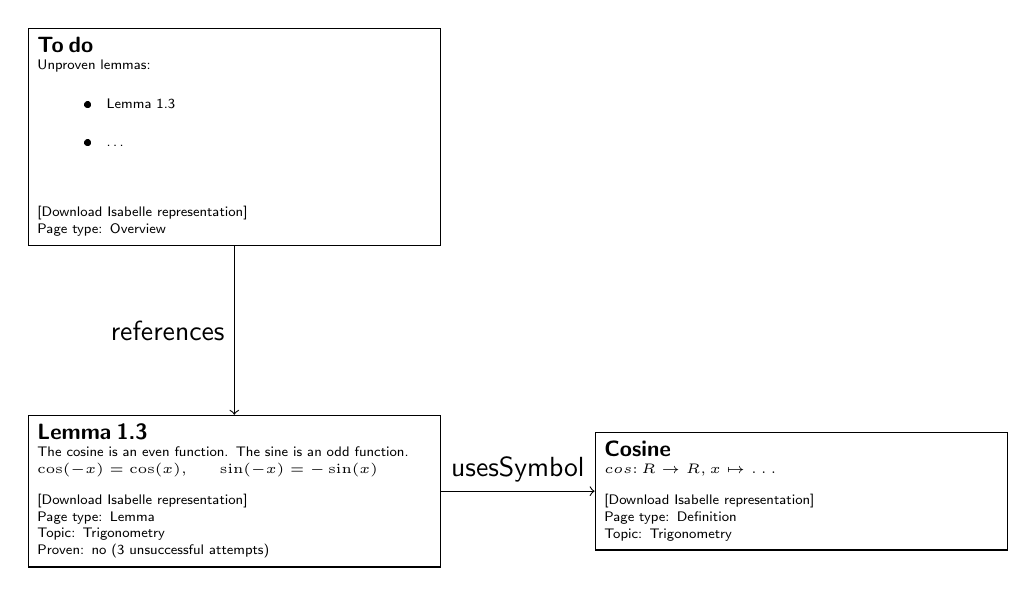
\begin{tikzpicture}[set style={{default}+=[scale=1.5,font=\sffamily]},default,xscale=.8]
    \wikipage{lemma}{(0,0)}{Lemma 1.3}{The cosine is an even function.  The sine is an odd function.\\
      $\cos(-x)=\cos(x),\qquad\sin(-x)=-\sin(x)$}{Page type: Lemma\\
      Topic: Trigonometry\\
      Proven: no (3 unsuccessful attempts)}
    \wikipage{cos}{(6,0)}{Cosine}{$cos\colon\mathbb{R}\to\mathbb{R},x\mapsto\ldots$}{
      Page type: Definition\\
      Topic: Trigonometry
    }
    \wikipage{todo}{(0,3)}{To do}{Unproven lemmas:
      \begin{itemize}
      \item Lemma 1.3
      \item \ldots
      \end{itemize}
    }{
      Page type: Overview
    }
    \draw[->] (lemma) -- node[above] {usesSymbol} (cos);
    \draw[->] (todo) -- node[left] {references} (lemma);
  \end{tikzpicture}
  \caption{Page structure}
  \label{fig:pagestructure}
\end{figure}

In the following two sections, we evaluate SWiM 0.2 and a prototype based on Semantic
MediaWiki for their applicability to Flyspeck with regard to their support for
annotations, browsing, and querying.  For the case study, we had the {\TeX} sources of the
Flyspeck book and a Twelf formalization of the first chapter (Trigonometry) at our
disposal.\ednote{@Sean/Florian: One/two sentences about Twelf!}  Currently we are
investigating whether Twelf is actually appropriate for formalizing Flyspeck.  We are also
investigating Isabelle, but we consider the design of the wiki support to be largely
independent of that decision.  After ???\ednote{@Sean: insert number} years, we consider
the basic narrative structure of the book a sufficiently stable for modeling the structure
of the wiki after it.  During the formalization of the knowledge, we anticipate that
mainly its axiomatic parts (i.\,e.\ the way concepts are defined) will undergo major
refactoring in order to facilitate the actual development of the proofs, as certain areas
of mathematics the Kepler proof heavily relies on, such as geometry, are underrepresented
in the existing formal mathematical libraries of theorem provers\ednote{@Sean: this is in
  a nutshell what you once told me about this; is it sufficient?}.  Additional refactoring
support by the wiki would thus be of advantage.

Secondly, we have not yet committed to a definitive workflow for formalizing the book.
Given the size of the book, which is much smaller than the size of the final
proofs\ednote{@Sean: right?}, the current Flyspeck core team may be able to create formal
representations of the symbol declarations, definitions, and lemmas manually and upload
them to the wiki.  On the other hand, wikis support a workflow where different groups of
authors, such as domain experts or proof-readers, collaborate in formalizing knowledge
step by step.  This potential could also be unleashed for Flyspeck.

%%% Local Variables: 
%%% mode: latex
%%% fill-column: 90
%%% TeX-master: "flyspeck-wiki-eswc08"
%%% End: 
